\documentclass[10pt]{article}

%% Load the ScAI template package
%% Use \usepackage[final]{scai} to remove all review annotations
\usepackage{scai}

%% Additional packages (add your own as needed)
\usepackage[authoryear, sort&compress, round]{natbib}
\usepackage{booktabs}
\usepackage{multirow}
\usepackage{subcaption}
\usepackage{algorithm}
\usepackage{algpseudocode}
\usepackage{cleveref}
\usepackage{bm}
\usepackage{lipsum}
\usepackage{tikzducks}
\usepackage{adjustbox}

%% Review annotators (removed automatically with \usepackage[final]{scai})
\annotator{alice}{red}
\annotator{bob}{blue}

%% ============================================================
%% Paper metadata
%% ============================================================

\title{Your Paper Title Goes Here}

%% Contribution notes — define BEFORE authors so symbols resolve correctly
%% Two formats supported:
%%   \contribnote{key}{description}            — auto-assigns footnote symbols (*, †, ‡, §, ...)
%%   \contribnote{key}{\symbol}{description}   — explicit symbol
\contribnote{equal}{Equal contribution.}              % auto-assigned: *
\contribnote{corr}{\ddag}{Corresponding author.}      % explicit symbol: ‡

%% Authors — \scaiauthor{affil,contribkeys}{Name}
%% Multiple affiliations: \scaiauthor{1,2,equal}{Name} produces Name^{1,2,*}
\scaiauthor{1,equal}{First Author}
\scaiauthor{1,2,equal}{Second Author}
\scaiauthor{2}{Third Author}
\scaiauthor{1,corr}{Corresponding Author}

%% Affiliations
\affiliation{1}{University of California, Los Angeles}
\affiliation{2}{Another University}

%% Keywords (optional — comment out to hide)
\scaikeywords{Keyword One, Keyword Two, Keyword Three}

%% Optional metadata fields (comment out any you don't need)
\correspondence{Corresponding Author}{corresponding@cs.ucla.edu}
\metadata[Date]{\today}
\metadata[Code]{\url{https://github.com/your-repo}}
\metadata[Data]{\url{https://your-data-url}}
\metadata[Website]{\url{https://your-website}}

%% Abstract
\begin{abstract}
This is a sample document demonstrating the UCLA ScAI lab paper template.
The template provides a clean, single-column layout with UCLA blue section headings,
Arial/Helvetica for titles and headings, Times New Roman for body text,
and Computer Modern for equations. It supports flexible author annotations,
affiliations, contribution notes, and optional metadata fields.
Replace this text with your own abstract.
\end{abstract}

%% Report number (optional, for internal tracking)
% \reportnumber{001}

%% ============================================================
%% Document body
%% ============================================================

\begin{document}
\maketitle

\section{Introduction}

Recent advances in large language models \citep{brown2020language} have enabled new capabilities across a wide range of tasks. Building on the transformer architecture \citep{vaswani2017attention}, these models can be further improved through reinforcement learning techniques such as proximal policy optimization \citep{schulman2017proximal}.

\lipsum[1]

\subsection{Related Work}

\lipsum[3]

\subsubsection{A Subsubsection}

\lipsum[4]

\section{Method}

Consider a dataset $\mathcal{D} = \{(\bm{x}_i, y_i)\}_{i=1}^{N}$ where $\bm{x}_i \in \mathbb{R}^d$ are input vectors and $y_i \in \mathcal{Y}$ are labels. Let $\bm{W} \in \mathbb{R}^{m \times d}$ be a weight matrix, $\bm{b} \in \mathbb{R}^m$ a bias vector, and $\bm{\theta} = \{\bm{W}, \bm{b}\}$ the set of all parameters. The model computes $\bm{h} = \sigma(\bm{W}\bm{x} + \bm{b})$ where $\sigma$ is a nonlinearity.

The training loss is:
\begin{equation}
    \mathcal{L}(\bm{\theta}) = \mathbb{E}_{(\bm{x}, y) \sim \mathcal{D}} \left[ \ell(f_{\bm{\theta}}(\bm{x}), y) \right].
    \label{eq:loss}
\end{equation}

The conditional probability of an action given a state is written as $\pi_{\bm{\theta}}(a \mid s)$, and the policy gradient is:
\begin{equation}
    \nabla_{\bm{\theta}} J(\bm{\theta}) = \mathbb{E}_{\tau \sim \pi_{\bm{\theta}}} \left[ \sum_{t=0}^{T} \nabla_{\bm{\theta}} \log \pi_{\bm{\theta}}(a_t \mid s_t) \, A^{\pi}(s_t, a_t) \right],
    \label{eq:pg}
\end{equation}
where $A^{\pi}(s_t, a_t)$ is the advantage function. Note the use of $\mid$ for conditioning (e.g., $p(y \mid \bm{x})$) versus $|$ for absolute value (e.g., $|\mathcal{D}|$).

We optimize \Cref{eq:loss} using gradient descent, as outlined in \Cref{alg:training}. Results are shown in \Cref{tab:results} and \Cref{fig:example}.

\begin{algorithm}[htbp]
    \caption{Example Training Procedure}
    \label{alg:training}
    \begin{algorithmic}[1]
        \Require Dataset $\mathcal{D}$, learning rate $\alpha$, epochs $T$
        \Ensure Trained parameters $\bm{\theta}^*$
        \State Initialize parameters $\bm{\theta}_0$ randomly
        \For{$t = 1$ to $T$}
            \For{each mini-batch $(\bm{x}, y) \sim \mathcal{D}$}
                \State Compute loss $\mathcal{L}(\bm{\theta}) \gets \ell(f_{\bm{\theta}}(\bm{x}), y)$
                \State Update $\bm{\theta} \gets \bm{\theta} - \alpha \nabla_{\bm{\theta}} \mathcal{L}(\bm{\theta})$
            \EndFor
            \If{validation loss converges}
                \State \textbf{break}
            \EndIf
        \EndFor
        \State \Return $\bm{\theta}^* \gets \bm{\theta}$
    \end{algorithmic}
\end{algorithm}

\begin{table}
    \centering
    \begin{tabular}{lcc}
        \toprule
        Method & Accuracy & F1 Score \\
        \midrule
        Baseline & 85.2 & 84.1 \\
        Ours & \textbf{91.7} & \textbf{90.3} \\
        \bottomrule
    \end{tabular}
    \caption{Example results table.}
    \label{tab:results}
\end{table}

\begin{figure}
    \centering
    \adjustbox{width=0.5\linewidth}{%
      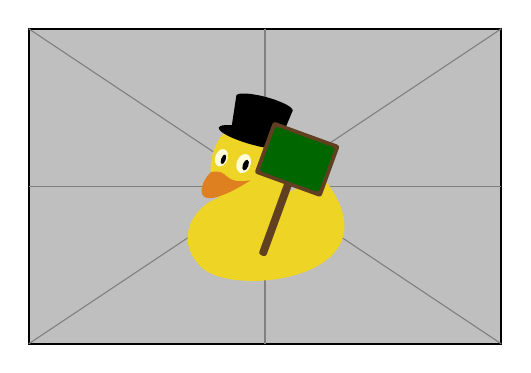
\begin{tikzpicture}
        \draw[black,fill=gray!50,thick] (0,0) rectangle (6,4);
        \draw[gray] (0,0) -- (6,4);
        \draw[gray] (0,4) -- (6,0);
        \draw[gray] (3,0) -- (3,4);
        \draw[gray] (0,2) -- (6,2);
        \node at (3,2) {\tikz\randuck;};
      \end{tikzpicture}
    }
    \caption{Example figure with a duck. Replace with your own figure.}
    \label{fig:example}
\end{figure}

\section{Experiments}

\lipsum[6-7]

\section{Conclusion}

\lipsum[8]

%% Example review annotations (removed with [final] option)
\alice{This paragraph needs more detail on the experimental setup.}
\alice[del]{This sentence is redundant and should be removed.}
\bob{Looks good to me.}

\bibliographystyle{plainnat}
\bibliography{references}

%% ============================================================
%% Appendix
%% ============================================================
%% Start appendix with centered title and table of contents
%% Default title: "Supplementary Materials"; customize with \makeappendixtitle[Your Title]
\makeappendixtitle

\section{Additional Experimental Details}
\label{app:details}

\subsection{Hyperparameters}
\label{app:hyperparams}

\lipsum[9]

The supplementary equation below is numbered with the ``S'' prefix:
\begin{equation}
    \nabla_{\bm{\theta}} J(\bm{\theta}) = \mathbb{E}_{\tau \sim \pi_{\bm{\theta}}} \left[ \sum_{t=0}^{T} \nabla_{\bm{\theta}} \log \pi_{\bm{\theta}}(a_t \mid s_t) \, A^{\pi}(s_t, a_t) \right].
    \label{eq:supp-pg}
\end{equation}

\begin{table}[htbp]
    \centering
    \begin{tabular}{lcc}
        \toprule
        Hyperparameter & Value & Description \\
        \midrule
        Learning rate & $3 \times 10^{-4}$ & Adam optimizer \\
        Batch size & 64 & Per GPU \\
        Epochs & 100 & Total training \\
        \bottomrule
    \end{tabular}
    \caption{Supplementary hyperparameters. Note the table is numbered S1.}
    \label{tab:supp-hyper}
\end{table}

\subsection{Environment Setup}
\label{app:env-setup}

\lipsum[10]

\section{Additional Figures}
\label{app:figures}

\subsection{Qualitative Results}
\label{app:qualitative}

\lipsum[12]

\begin{figure}[htbp]
    \centering
    \adjustbox{width=0.4\linewidth}{%
      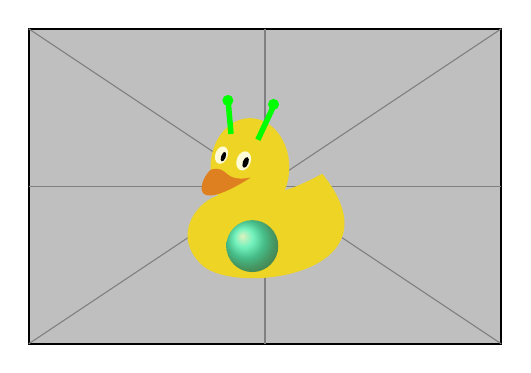
\begin{tikzpicture}
        \draw[black,fill=gray!50,thick] (0,0) rectangle (6,4);
        \draw[gray] (0,0) -- (6,4);
        \draw[gray] (0,4) -- (6,0);
        \draw[gray] (3,0) -- (3,4);
        \draw[gray] (0,2) -- (6,2);
        \node at (3,2) {\tikz\randuck;};
      \end{tikzpicture}
    }
    \caption{A supplementary duck figure. Note the figure is numbered S1.}
    \label{fig:supp-duck}
\end{figure}

\subsection{Training Curves}
\label{app:training-curves}

\lipsum[13]

\section{Proof of Main Theorem}
\label{app:proof}

\lipsum[11]

\end{document}
